\section{Logging}
\label{sec:module.Logging}

\section{JavaScript Addon f�r HMTL-Gameviewer}
\label{sec:implementation.Addon}
Das Codepaket welches von den Challenge-Organisatoren mitgeliefert wird, bietet bereits eine hilfreiche 2D-Visualisierung des Spiels, mit welchem das Spielgeschehen mitverfolgt werden kann. Die Visualisierung wurde mit HMTL und Javascript implementiert. Leider ist es nicht m�glich zus�tzliche Informationen auf die Seite zu projizieren. Deshalb haben wir den Viewer mit einer solchen Funktion erweitert. Mit der Codezeile Logger.liveInfo(...) kann eine Zusatzinformation geschrieben werden. Es muss definiert werden mit welchem Zug und wo auf dem Spielfeld die Infomation angezeigt werden soll. Im Beispiel wird an der Position der Ameise ausgegeben welchen Task die Ameise hat.
\begin{verbatim}
Logger.liveInfo(Ants.getAnts().getTurn(), ant.getTile(), 
                "Task: %s ant: %s", issuer, ant.getTile());
\end{verbatim}
Auf der Karte wird ein einfaches aber praktisches Popup mit den geschriebenen Informationen angezeigt. Dank solcher Zusatzinformationen muss nicht m�hsam im Log nachgeschaut werden, welcher Ameise wann und wo welcher Task zugeordnet ist.

\begin{figure}[bth]
\centering
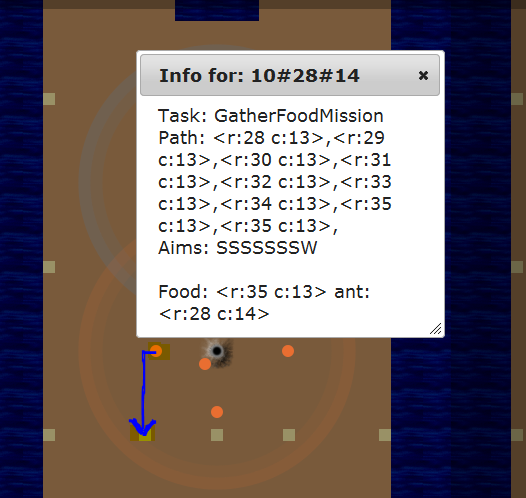
\includegraphics[height=70mm]{91_bilder/javascriptAddon.png}
\caption[Live-Info Popup]{Das Popup zeigt die Aufgabe und den Pfad (blau), welcher die Ameise ablaufen wird.}
\label{fig.javascriptAddon}
\end{figure}

Das angezeigte Popup zeigt welchen Task (GatherFoodTask) die Ameise hat, wo sie sich befindet <r:28 c:14>, welches Futterpixel angesteuert wird <r:35 c:13> und welchen Pfad dazu berechnet wurde. 